\section{The Symmetry Breaking Problem}
\label{cap:2}

Formally, a symmetry system can be defined as a system in which the processes are in an equivalence relation, this means that if the processes run the same code, it is possible to permute the processes without changing the behaviour of the system. One example of this state would be a ring in which there is no unique identifier for every processes \cite{boldi1996symmetry}. 

If we consider a message passing system in which exist an initial state of symmetry between all processes, it is possible to find a synchronous execution in which the processes will continue in the same initial state. In this case, it is necessary a mechanism to break the symmetry, on the contrary, the system cannot escape from the initial state.
%as shown in \cite{angluin1980local} by Angluin.

Symmetry breaking is one of the most extensively studied problems in distributed computing. The fundamental problems on graph include the maximal matching, vertex colouring, ruling sets and \textit{MIS}. The last one can be considered as the central problem because all the others can be reduced to it, as shown in  \cite{linial1992locality}.

In the next section, a formal definition of the maximal independent set is given. A  discussion on the sequential algorithm vs distributed algorithm is presented with the theoretical analysis on time complexity and message complexity in the case of the distributed approach. Henceforth the terms vertices and processes are used in the same context and are interchangeable.    

\subsection{Maximal Independent Set}

\theoremstyle{definition}
\begin{definition}

Given a undirected graph $G = (V,E)$, a Maximal Independent Set \textbf{MIS} is a set of vertices $S \subseteq V$ if it satisfied the following properties:   

\begin{enumerate}
  \item the set S in an independent set meaning that no two vertices $v,u \in S$ are adjacent,
  \item the set S is maximal, with regards to independence, meaning that for each vertex $v \notin S$, there exist a neighbour $u$ of $v$ such that $u \in S$.
\end{enumerate}

\end{definition}

REWRITE THIS PARAGRAPH
Figure \ref{fig:graph1} show an example of undirected graph $G$ with 8 vertices and 14 edges. The goal is to find a MIS of $G$, informally, a set of vertices in which every vertex $v$ is part of the set or a neighbour of $v$ is part of the set. It is possible to find more that one solution to the same instance as shown in the example.
 
\begin{figure}[ht]
\centering
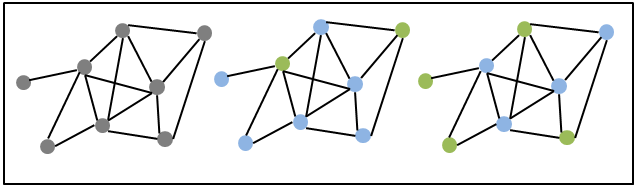
\includegraphics[width=1 \linewidth, height=5cm]{mis-example.PNG} 
\caption{Maximal Independent Set of a general graph}
\label{fig:graph1}
\end{figure}


The algorithm \ref{algorithm:secuential-mis} describe a general sequential algorithm to find the maximal independent set of a general graph. The time complexity is $O(N)$ since in the worst case, the algorithm has to check every vertex. Another approach to improve this time is desirable. In the next section, two distributed algorithm to find the \textit{MIS} are presented.

\begin{algorithm}
 \caption{Sequential Maximal Independent Set}
 \label{algorithm:secuential-mis} 

\SetAlgoNoLine
\KwResult{IS Set of vertices}
\KwData{ $G(V,E)$ Graph}
    \While {V is not empty}{
        Choose a vertex $v \in V$
            Add v to the set IS\;
            Remove from V the vertex v and all its neighbours\;
        }
    
 
\end{algorithm}
 
 


 
\subsection{Distributed Maximal Independent Set}

A logarithmic lower bound is always desirable to solve a problem optimally, for this reason, the difficulty to find it in sequential algorithms motivated the proposal of distributed algorithms. In distributed computing, randomised algorithm is a powerful and efficient technique to solve efficiently problem that may take longer time in deterministic approach.

In 1986, a efficient distributed algorithm was proposed independently by Luby \cite{luby1986simple} and Alon \textit{et al.} \cite{alon1986fast}. Both algorithms are randomised and have $O(log N)$ lower bound. Until now, there are faster than the best deterministic algorithms for general graphs. There have been some improvements for special cases, for instance, \cite{panconesi1996complexity} propose a $O(\delta + log^* N)$ algorithm for specific graphs, however, the original algorithms are still faster when the running time is expressed as a function of $N$. It is worth to mention that all algorithms exposed forward are in the synchronous model.  

The algorithm\ref{algorithm:luby-mis} describe the original Luby's algorithm. Show the correctness of this algorithm is very simple. In each round, if a vertex joins the set \textit{S}, no other neighbour join the set in the actual round or in any other round. The algorithm at the end produces a \textit{MIS} because the vertices with the highest degree will decide to enter the \textit{MIS} in each round until all vertices become inactive.

% If Luby’s algorithm ever
% terminates, then the final set S satisfies the
% independence property.

% Theorem 6: If Luby’s algorithm ever
% terminates, then the final set S satisfies the
% maximality property.

% \theoremstyle{definition}
\begin{definition}

An algorithm terminates w.h.p. (with high probability) within $O(t)$ time if it does so with probability at least $1 − 1/n^c$ for any choice of $c ≥ 1$.

\end{definition}

 Message complexity depends on the number of processes which are active in each phase and its denoted by $O(m)$ in \cite{luby1986simple}. With high probability $(1-1/n)$, the Luby's algorithm finishes  $4\log N$ round. 

% \theoremstyle{theorem}
\begin{theorem}

Algorithm \ref{algorithm:luby-mis} computes a maximal independent set for any graph  in $O(\log n)$  rounds with high probability.

\end{theorem}


\begin{algorithm}
 \caption{Luby's Algorithm, code for each process $p_i$ i = 1 to N}
 \label{algorithm:luby-mis} 

\SetAlgoNoLine
\KwResult{MIS Maximal Independent Set}
\KwData{ $G(V,E)$ Graph}
    \While {V is not empty}{
        Choose a random set of vertices $S ⊆ V$, by selecting each vertex $v$ independently with probability $1/(2d(v))$, where d is the degree of $v$\;
        For every edge in E, if both its endpoints are in the random set S, then remove from S the endpoint whose degree is lower. Break ties arbitrarily, e.g. using a lexicographic order on the vertex names\;
        Add the set S to IS\;
        Remove from V the set S and all the neighbours of vertices in S\;
        }
\end{algorithm} 



The algorithm \ref{algorithm:main-mis} is another randomized distributed algorithm and was proposed by Yves \cite{yves2009optimal}. This algorithm is used for the simulations in this project. The rounds can be split into 2 phases for simplicity. In each phase, each process chooses a random value, send to its neighbours and wait to receive the value from all its neighbours. If the process has the maximum value, the join the set and output in. In the second phase, if the process decided to join the $MIS$, then send messages to all its actives neighbours. If the process receives a message from one neighbour, decide not join the MIS and output out. At the end of this phase, every process that made a decision about join or not the \textit{MIS} become inactive for the next rounds.

\begin{algorithm}
 \caption{MIS Algorithm, code for each process $p_i$ from $i = 1$ to $N$}
 \label{algorithm:main-mis} 

\SetAlgoNoLine
\KwResult{MIS Maximal Independent Set}
\KwData{ $G(V,E)$ Graph}
    \While {V is not empty}{
        Selects a random number $r(v)$ between [0,1] and sends to its neighbours\;
        If $r(v) < r(w)$ for all neighbours $w \in N(v)$ numbers, remove myself from V and enter to the MIS \newline
        Inform my neighbours that I am a MIS member and terminate\;
        If I heard that my neighbour is MIS, remove myself from the V and terminate\;
        }
\end{algorithm}

% Lemma 7.14 (Edge Removal). In a single phase, we remove at least half of
% the edges in expectation.

The correctness is very intuitive and similar to the Luby's algorithm. In one phase, one process $p_i$ join the set $S$ only if it has the larger value between its neighbours, at the end of that phase, all the $p_i$ neighbours become inactive. In consequence, there is no neighbour process in the $S$. This set $S$ is maximal because at least one vertex (with the global smallest value) will enter the $S$ per round, hence there is a progress in each round. If at some round, a vertex has no neighbours, automatically join $S$ and become inactive. This sequence continues in following rounds until every process becomes inactive

% \theoremstyle{theorem}
\begin{theorem}

Algorithm \ref{algorithm:main-mis} computes a maximal independent set for any graph in $O(\log n)$ rounds with high probability.

\end{theorem}


% . This algorithm operates in synchronous rounds. In line 2, every process select a random number to in order to break the symmetry with its neighbours, line 3 makes sure that if a vertex v join the MIS, no other neighbour of v join the MIS at the same time, this is true because the execution  occurs in rounds. the line 4 makes sure that any vertex that has a neighbour in the MIS, join the MIS at any point. 


\newpage